\paragraph{}
Pour valider la réalisation des besoins fonctionnels et non fonctionnels présentés dans le cahier des charges, une série de tests a été effectuée sur le logiciel.

\subsubsection{Tests fonctionnels}
\paragraph{}
Concernant les besoins fonctionnels, nous avons manipulé le logiciel sous les différents systèmes d'exploitation envisagés, à savoir Windows et Linux. Les procédures de tests ont été listées en Annexe.
Les différentes rotations de la caméra autour de la scène ont bien été implémentées, permettant à l'utilisateur de voir les objets qui y sont placés sous différents angles, et de s'en rapprocher ou de s'en éloigner grâce au zoom. La translation de la caméra a également été implémentée, même si son utilisation nécessite une souris.
Les objets sont issus de fichiers d'extension OBJ version 3.0, ASCII, ou PLY, versions 1.0, ASCII et binaire. Ceux-ci peuvent ensuite être sélectionnés un par un, en cliquant sur la scène ou sur son nom dans la liste des objets. L'utilisateur peut alors les déplacer grâce à des translations et rotations selon trois axes, et modifier leur taille. Ils pourront également être supprimés de la scène.
Enfin, les différents rendus prévus ont pu être obtenus à partir de la scène. Pour chacun d'entre eux, une nouvelle fenêtre est ouverte, proposant les paramètres modifiables pour la génération des photographies, anaglyphes, autostéréogrammes, et folioscopes. Pour chacun d'entre eux, on proposera une prévisualisation, et la possibilité d'enregistrer les images intermédiaires ayant permis ce résultat, à savoir les vues gauche et droite pour les anaglyphes, la carte des profondeurs pour les autostéréogrammes, et chaque image du folioscope permettant d'obtenir un GIF animé.
Comme prévu, même si l'utilisateur ne demande pas d'enregistrer la scène, une sauvegarde automatique a été mise en place à intervalles de temps régulier. Elle permet de s'assurer que même en cas d'arrêt non souhaité du logiciel, seules les dernières modifications seront perdues.

\subsubsection{Tests de validation}
\paragraph{}
Les tests des besoins non fonctionnels ont permis de valider la portabilité et la fluidité du logiciel. L'extensibilité du logiciel aura été permise par l'architecture du logiciel, qui a été présentée dans la partie Réalisation du projet.

\paragraph{}
Pour s'assurer de la portabilité du logiciel, nous avons effectué les manipulations de tests des besoins fonctionnels sur les différentes machines de notre équipe de programmeur. Ces machines utilisent les systèmes d'exploitation Linux et Windows, et possèdent soit une carte graphique soit un chipset graphique. Les machines de tests possédant une carte graphique sont données dans la figure \ref{fig:machines_cg}.

\begin{figure}[h]
  \begin{changemargin}{-4cm}{-4cm}
    \centering
    \begin{tabular}{|l|c|c|c|}
      \hline
      Système d'exploitation & Système graphique & Mémoire RAM \\ \hline \hline
      Windows 7 IntelCore I7 64bits & NVIDIA GetForce GTX 770 & 8Go DDR3 \\ \hline
      Windows 7 IntelCore I5 64bits & NVIDIA GetForce GTX 760 & 8Go DDR3 \\ \hline
    \end{tabular}
  \end{changemargin}
  \caption{Machines de tests avec carte graphique}
  \label{tab:machines_cg}
\end{figure}

Les machines de tests possédant un chipset sont données dans la figure \ref{machines_chip}.

\begin{figure}[h]
  \begin{changemargin}{-4cm}{-4cm}
    \centering
    \begin{tabular}{|l|c|c|c|}
      \hline
      Système d'exploitation & Système graphique & Mémoire RAM \\ \hline \hline
      Windows 7 IntelCore I5 64bits & Intel HD Graphics 4000 & 8GoDDR3 \\ \hline
      Fedora 21 IntelCore I3 64bits & Intel HD Graphics 4000 & 4GoDDR3 \\ \hline
    \end{tabular}
  \end{changemargin}
  \caption{Machines de tests avec Chipset graphique}
  \label{tab:machines_chip}
\end{figure}

\paragraph{}
La fluidité du logiciel a été testée grâce aux modèles happy.ply et blade.ply qui avaient servi de modèles lors de la réalisation du cahier des charges. Ces objets sont respectivement composés de 543 652 sommets et de 882 954 sommets. Les valeurs de frame par seconde (fps) ont été testées grâce au logiciel Fraps\footnotemark.
Sur une machine Windows disposant d'un chipset graphique, on obtient des résultats allant entre 30 et 55 fps pour ces deux modèles, comme le montre la figure \ref{fig:fps_windows_chipset}. 
\footnotetext{\url{http://www.fraps.com/}}

\begin{figure}[h]
	\centering
	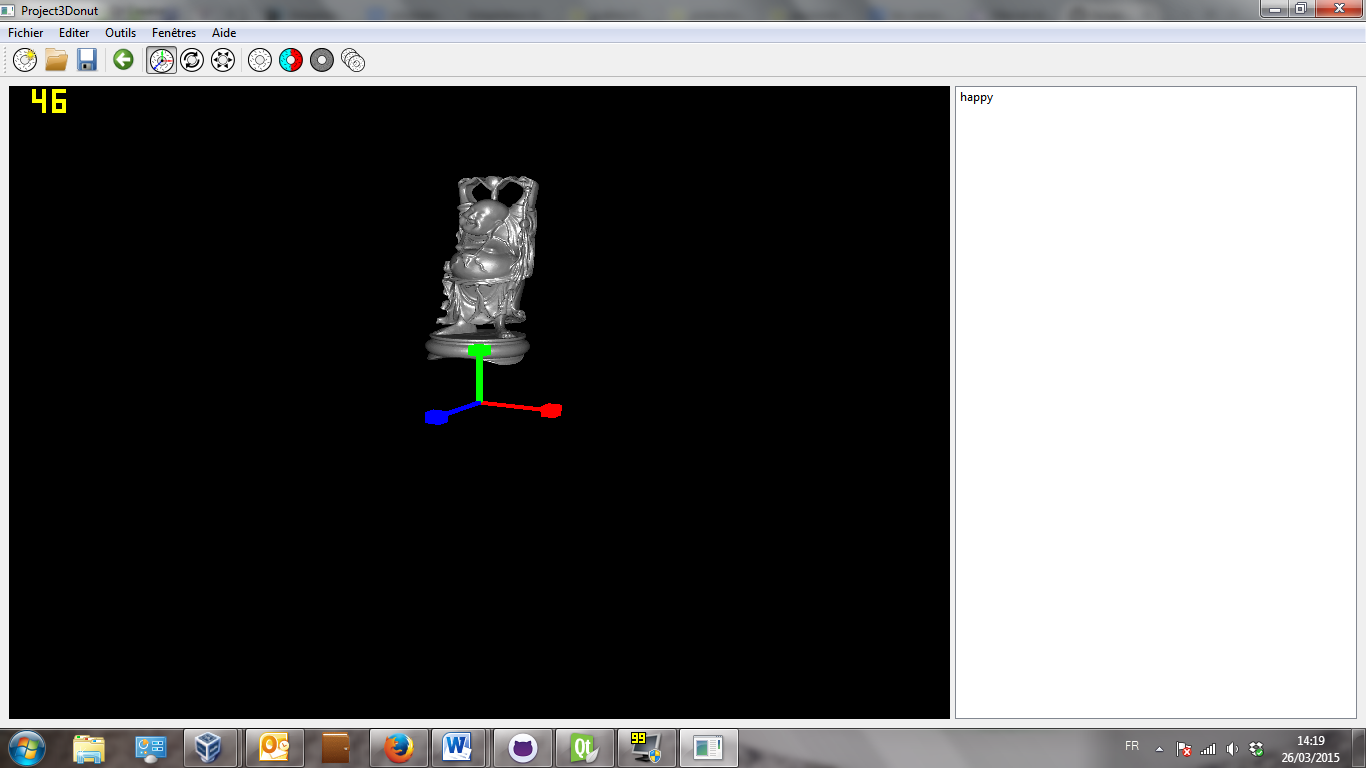
\includegraphics[scale=0.3]{happy_fps.png}
        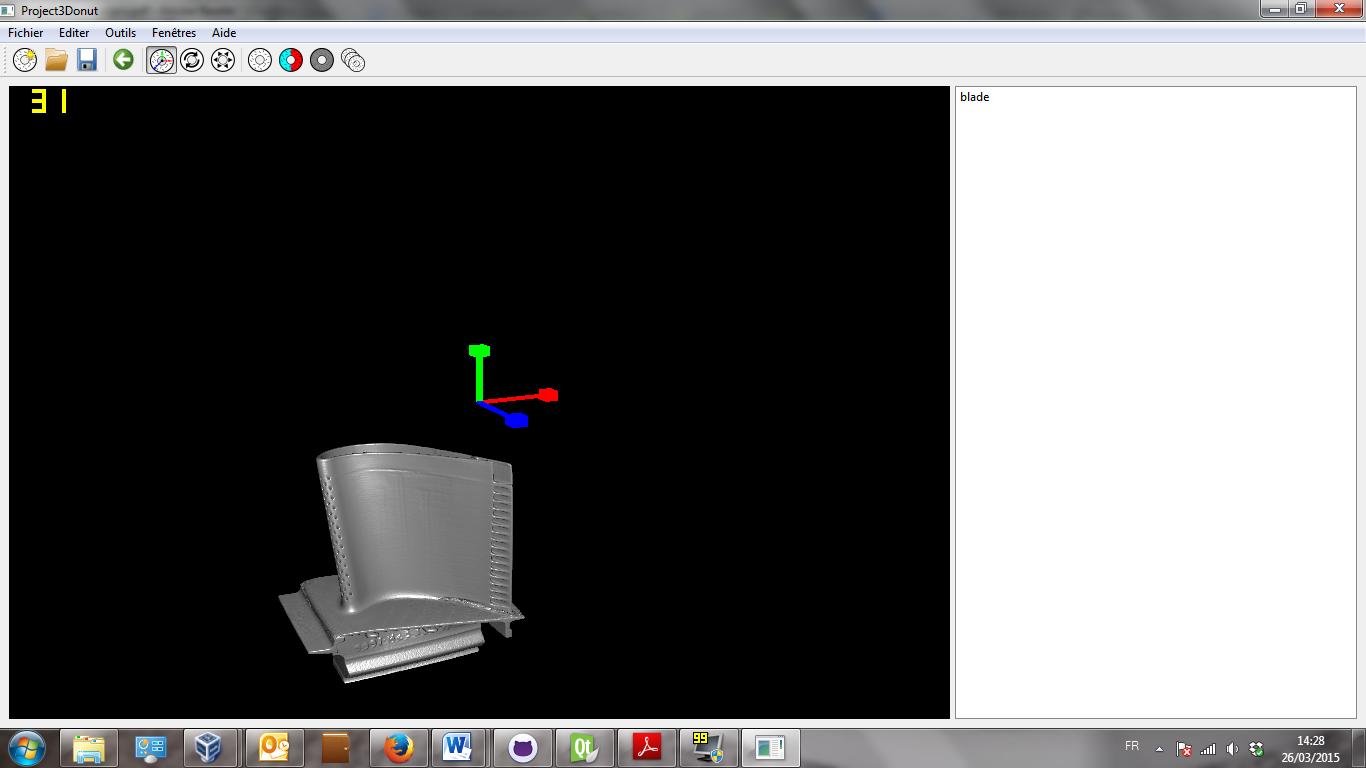
\includegraphics[scale=0.3]{blade_fps.png}
       	\caption{\label{fig:fps_windows_chipset} Test de fps sur une machine Windows avec chipset graphique\protect}
\end{figure}
[RESULTATS WINDOWS/LINUX/CHIPSET]
[RESULTAT SANS CHIPSET]

Le cahier des charges prévoyaient un affichage de 25fps pour un nombre de sommets au moins cinq fois inférieur à celui de 'happy.ply' (prévision de 25 fps pour 100 000 sommets avec un chipset graphique, alors qu'on en obtient cette fluidité pour plus de 500 000 points). Ce même test de fluidité a été réalisé sur d'autres machines de notre équipe, sur les modèles présentés dans la figure \ref{fig:modeles}. Les résultats sont donnés dans la figure \ref{fig:fps_cg} pour les machines avec carte graphique, et dans la figure \ref{fig:fps_chip} pour les machines avec chipset.

\begin{figure}[h]
  \begin{changemargin}{-4cm}{-4cm}
    \centering
    \begin{tabular}{|l|c|c|c|}
      \hline
      Nom du modèle & Nombre de sommets & Nombre de faces \\ \hline
      happy.ply & 543 652 & 1 087 716 \\ \hline
      blade.ply & 882 954 & 1 765 388 \\ \hline
    \end{tabular}
  \end{changemargin}
  \caption{Modèles testés lors de la fluidité d'affichage}
  \label{tab:modeles}
\end{figure}

\begin{figure}[h]
  \begin{changemargin}{-4cm}{-4cm}
    \centering
    \begin{tabular}{|l|c|c|c|}
      \hline
      Système d'exploitation & Windows 7 IntelCore I7 64bits & Windows 7 IntelCore I5 64bits & Windows 8 64bits\\ \hline
      Carte graphique &  NVIDIA GetForce GTX 770 & NVIDIA GetForce GTX 760 & GT360M \\ \hline
      Mémoire RAM & 8GoDDR3 & 8GoDDR3 & 4GoDDR3 \\ \hline \hline
      happy.ply & 60 & 60 & 84 \\ \hline
      blade.ply & 60 & 60 & 60\\ \hline
    \end{tabular}
  \end{changemargin}
  \caption{Test de fluidité sur les machines avec carte graphique}
  \label{tab:fps_cg}
\end{figure}

\begin{figure}[h]
  \begin{changemargin}{-4cm}{-4cm}
    \centering
    \begin{tabular}{|l|c|c|c|}
      \hline
      Système d'exploitation & Windows 7 IntelCore I5 64bits & Fedora 21 IntelCore I3 64bits & ArchLinux\\ \hline
      Chipset graphique &  Intel HD Graphics 4000 & Intel HD Graphics 40008GoDDR3 & Intel Mobile Series 4 \\ \hline
      Mémoire RAM & 8GoDDR3 & 4GoDDR3  & \\ \hline \hline
      happy.ply & 55 & 60 & 8\\ \hline
      blade.ply & 35 & 50 & 5\\ \hline
    \end{tabular}
  \end{changemargin}
  \caption{Test de fluidité sur les machines avec chipset graphique}
  \label{tab:fps_chip}
\end{figure}

\paragraph{}
L'ensemble de ces tests auront permis de s'assurer de la conformité de notre projet au Cahier des charges. 

\subsubsection{Test de charge}
Pour tester les limites de notre logiciel, nous avons choisi d'importer plusieurs exemplaires d'un même modèle, 'happy.ply' présenté dans la figure \ref{fig:modeles}, dans une scène. Les résultats de ce test de charge sont donnés dans la figure \ref{fig:charge_cg} pour les machines avec carte graphique, et dans la figure \ref{fig:charge_chip} pour les machines avec chipset.

\begin{figure}[h]
  \begin{changemargin}{-4cm}{-4cm}
    \centering
    \begin{tabular}{|l|c|c|c|}
      \hline
      Système d'exploitation & Windows 7 IntelCore I7 64bits & Windows 7 IntelCore I5 64bits & Windows 8 64 bits\\ \hline
      Carte graphique &  NVIDIA GetForce GTX 770 & NVIDIA GetForce GTX 760 & GT360M\\ \hline
      Mémoire RAM & 8GoDDR3 & 8GoDDR3 & 4GoDDR3 \\ \hline \hline
      543 652 sommets (1fois) & 60 & 60 & 84 \\ \hline
      1 087 304 sommets (2fois) & 60 & 60 & 44 \\ \hline
      1 630 956 sommets (3fois) & 60 & 60 & 30 \\ \hline
      2 174 608 sommets (4fois) & 60 & 60 & 23 \\ \hline
      2 718 260 sommets (5fois) & 60 & 60 & Out of Memory \\ \hline
      3 261 912 sommets (6fois) & 60 & 60 & Out of Memory \\ \hline
      3 805 564 sommets (7fois) & 60 & 60 & Out of Memory \\ \hline
      4 349 216 sommets (8fois) & Out of Memory & 60 & Out of Memory  \\ \hline
      4 892 868 sommets (9 fois) & Out of Memory & Out of Memory & Out of Memory \\ \hline
    \end{tabular}
  \end{changemargin}
  \caption{Test de charge sur les machines avec carte graphique}
  \label{tab:fps_cg}
\end{figure}

\begin{figure}[h]
  \begin{changemargin}{-4cm}{-4cm}
    \centering
    \begin{tabular}{|l|c|c|c|}
      \hline
      Système d'exploitation & Windows 7 IntelCore I5 64bits & Fedora 21 IntelCore I3 64bits & ArchLinux\\ \hline
      Chipset graphique &  Intel HD Graphics 4000 & Intel HD Graphics 4000 & Intel Mobile Series 4 \\ \hline
      Mémoire RAM & 8GoDDR3 & 4GoDDR3 & \\ \hline \hline
      543 652 sommets (1fois) & 55 & 60 & 8\\ \hline
      1 087 304 sommets (2fois) & 29 & 34 & Out of Memory\\ \hline
      1 630 956 sommets (3fois) & 20 & 22 & Out of Memory \\ \hline
      2 174 608 sommets (4fois) & 15 & 16 & Out of Memory \\ \hline
      2 718 260 sommets (5fois) & Out of Memory & 13 & Out of Memory \\ \hline
      3 261 912 sommets (6fois) & Out of Memory & 10 & Out of Memory \\ \hline
      3 805 564 sommets (7fois) & Out of Memory & 9 & Out of Memory \\ \hline
      4 349 216 sommets (8fois) & Out of Memory & 6 & Out of Memory \\ \hline
      4 892 868 sommets (9 fois) & Out of Memory & Out of Memory & Out of Memory \\ \hline
    \end{tabular}
  \end{changemargin}
  \caption{Test de charge sur les machines avec chipset graphique}
  \label{tab:fps_chip}
\end{figure}

\subsubsection{Tests de profilage}
\paragraph{}
Pour s'assurer de la qualité du code, nous avons choisi d'utiliser l'outil Valgrind. Celui-ci permet notamment de détecter des fuites mémoire dans le déroulement du logiciel. Si toutes n'ont pas pu être évitées, l'utilisation des \texttt{std::unique\_ptr} ont permis de s'assurer que certaines instances ne pouvaient pas être dupliquées. Nous avons ainsi pu éviter de nombreuses fuites mémoires.


